\documentclass[]{cph18}
\usepackage{amsmath}

\begin{document}

\title{Project title}
\author{Yangkang Chen$^*$, Zhejiang University\\
        Second author, Second institution}
\maketitle

\begin{abstract}
A brief summary of the work.
\end{abstract}

\newpage

\section{Introduction}

\section{Method}

\section{Synthetic data examples}

\section{Field data examples}

 
\section{Conclusions}


\section{Acknowledgements}



%\begin{figure}
%	\centering
%	\subfloat[]{\includegraphics[width=0.8\textwidth]{Fig/fig}}
%	\caption{Caption.}
%	\label{fig:fig}
%\end{figure}


%\begin{figure}
%	\centering
%	\subfloat[]{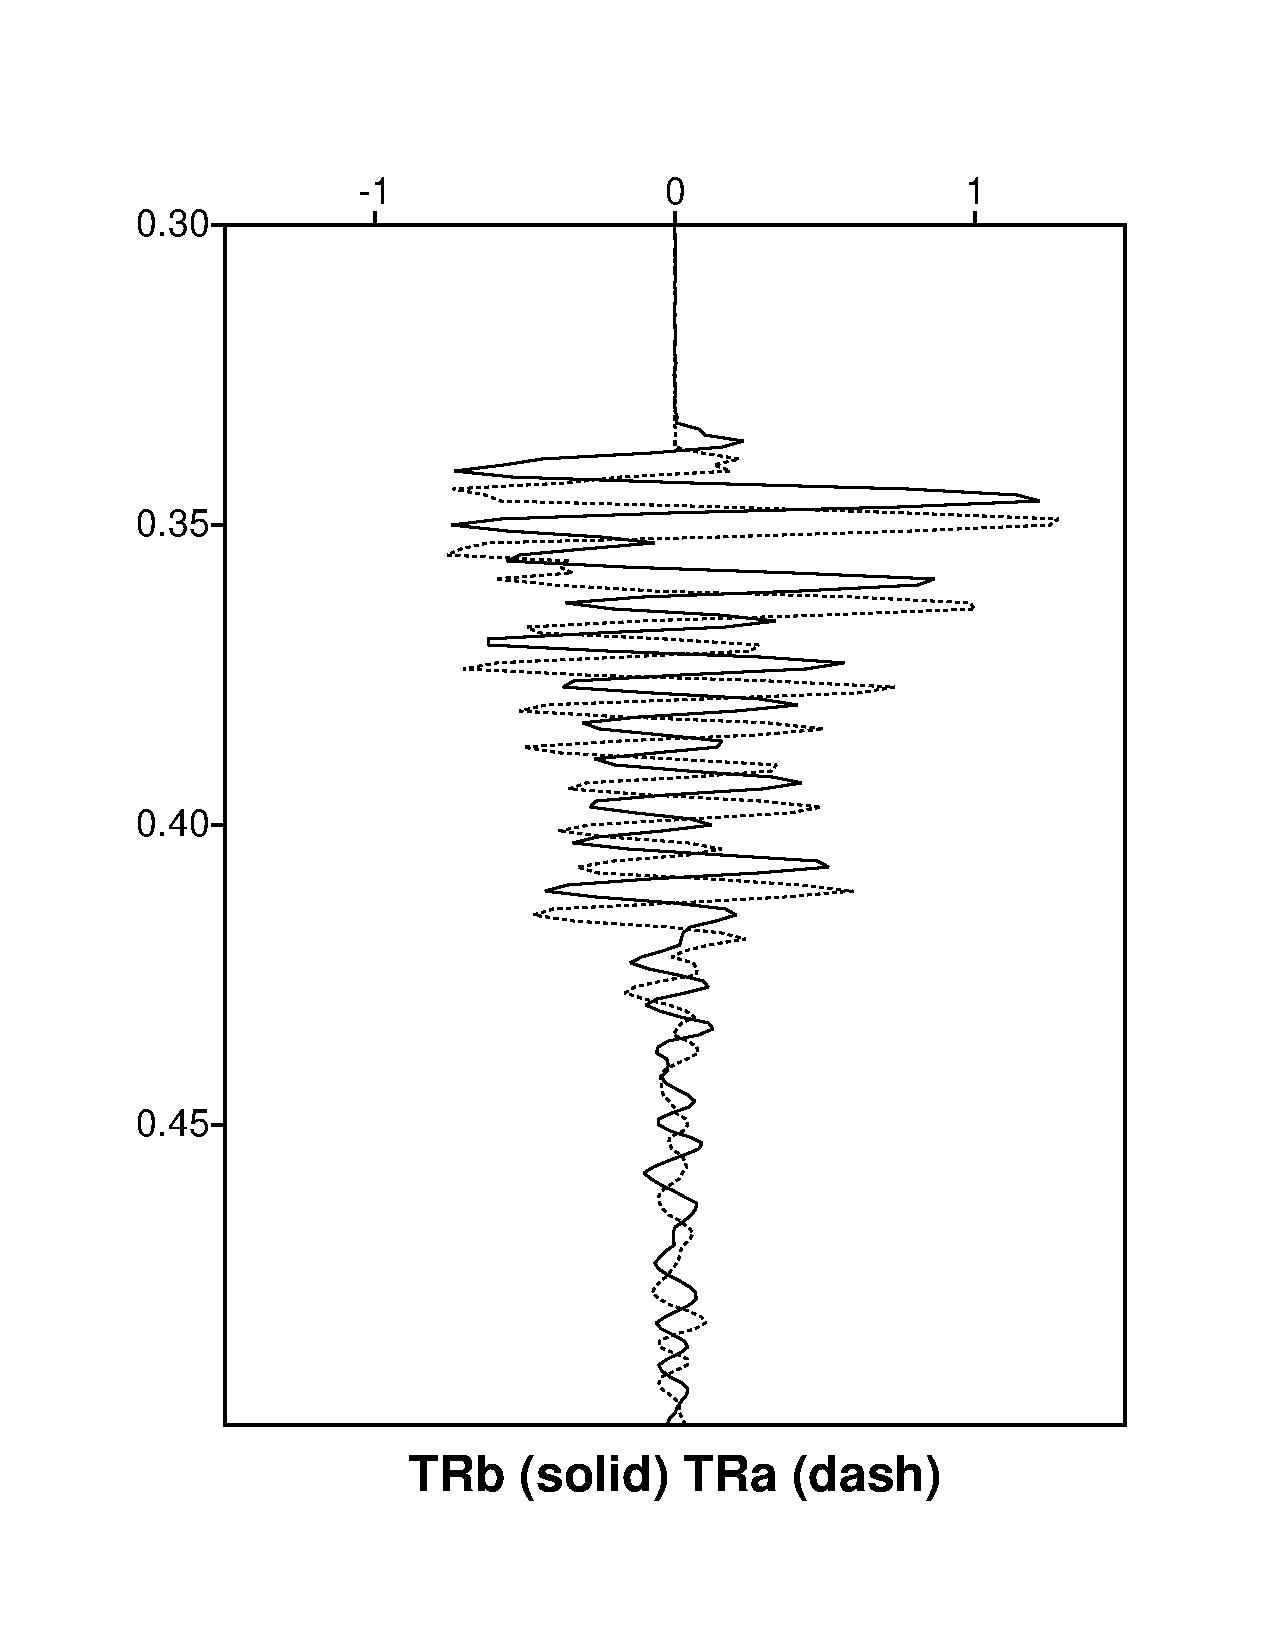
\includegraphics[width=0.45\textwidth]{Fig/fig1}}\\
%    \subfloat[]{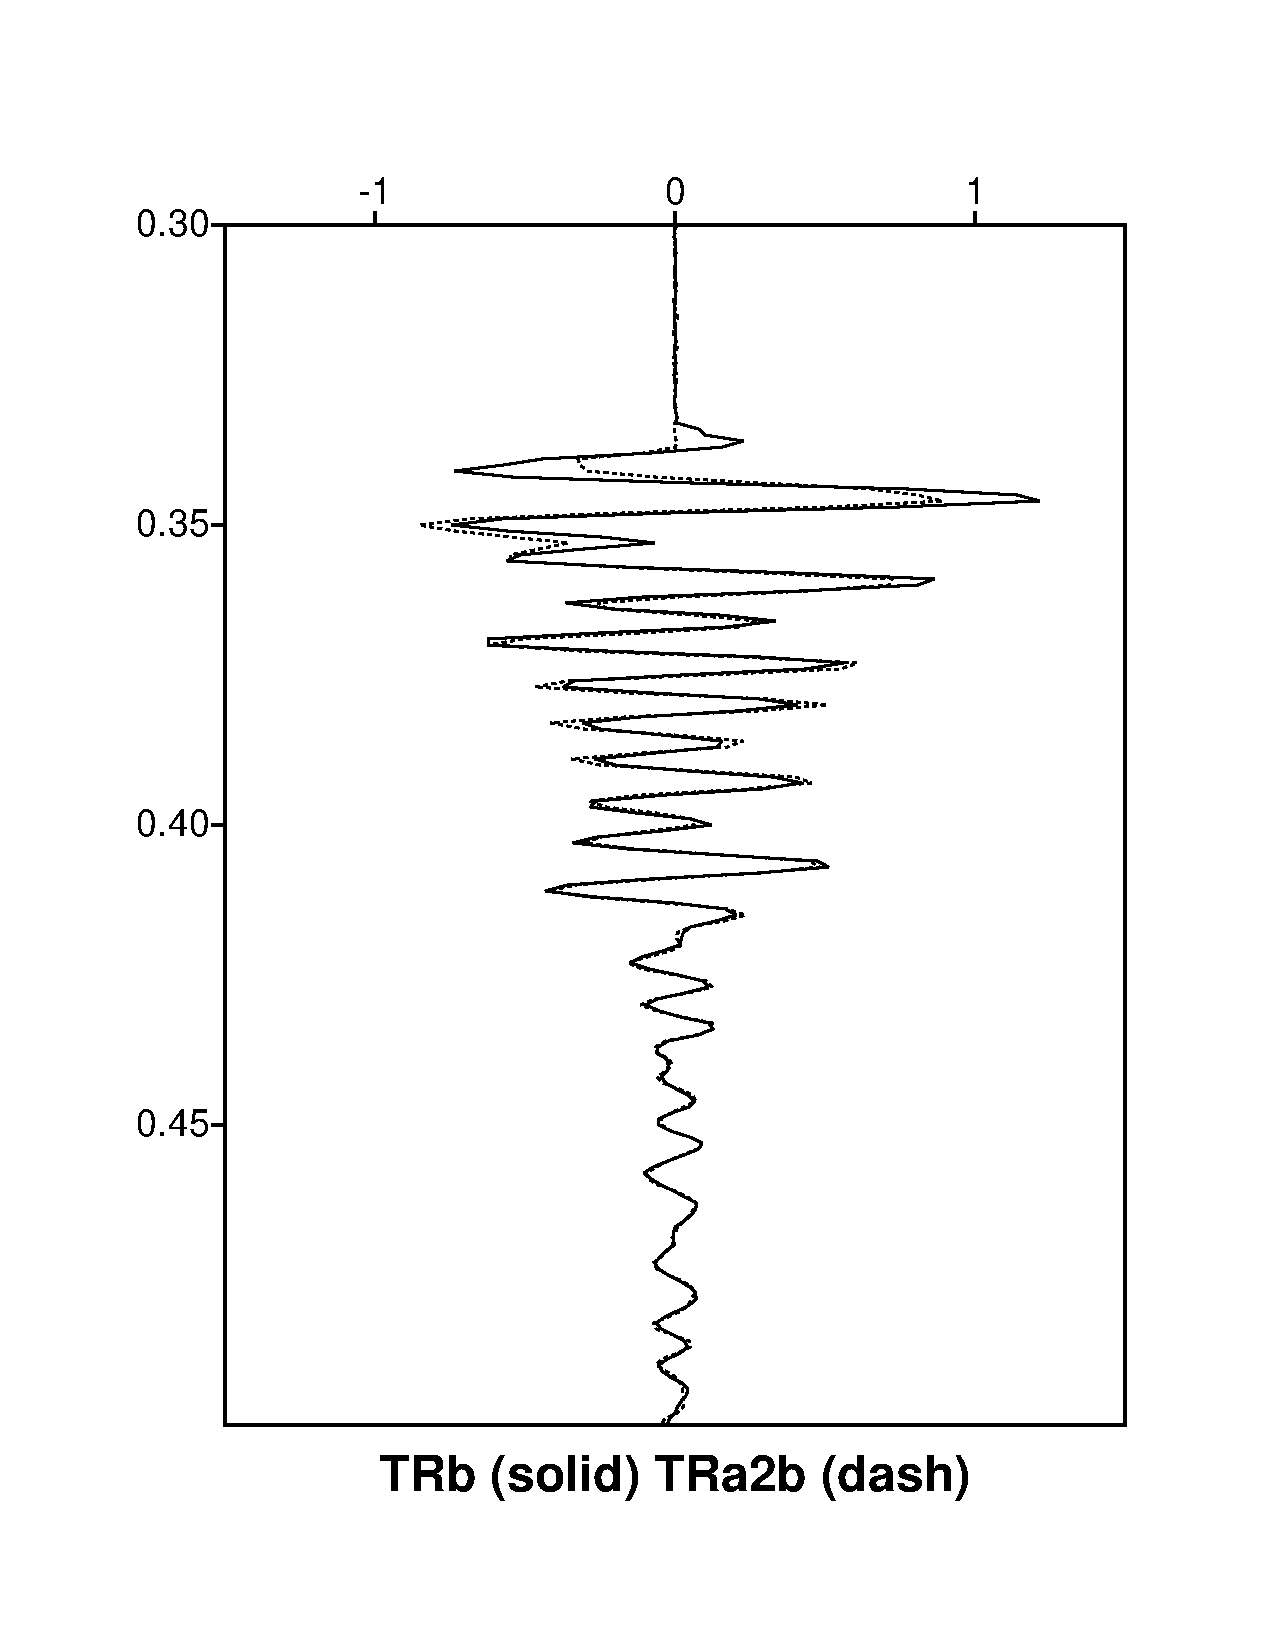
\includegraphics[width=0.45\textwidth]{Fig/fig2}}
%	\caption{(a) Caption a. (b) Caption b.}
%	\label{fig:fig1,fig2}
%\end{figure}


\bibliographystyle{firstbreak}
\bibliography{projname}

\end{document}























